%% =====================================================================
%% Artículo del proyecto de grado — Maestría en Inteligencia Artificial
%% Universidad de los Andes · Curso Proyecto: despliegue de soluciones
%% Plantilla: IEEEtran.cls v1.7a (modo conference), según el ejemplo
%% de la carpeta Ejemplo-Proyecto-LaTeX2e.
%%
%% Compilar:  pdflatex articulo.tex   (dos veces, para referencias cruzadas)
%%   o bien:  latexmk -pdf articulo.tex
%%
%% Los resultados que aún no existen están marcados con \pendiente{...}
%% (texto rojo). Antes de entregar: buscar "\pendiente" y reemplazar.
%% =====================================================================
\documentclass[conference,letterpaper]{IEEEtran}

% ---------- Codificación, idioma y tipografía ----------
\usepackage[T1]{fontenc}
\usepackage[utf8]{inputenc}
\usepackage{mathptmx}            % Times, como pide el formato del curso
% Español si está instalado babel-spanish; si no, se traducen los rótulos a mano.
\IfFileExists{spanish.ldf}{%
  \usepackage[spanish,es-tabla,es-nodecimaldot,es-noshorthands]{babel}%
}{%
  \usepackage[english]{babel}%
  \addto\captionsenglish{%
    \renewcommand{\figurename}{Figura}%
    \renewcommand{\tablename}{Tabla}%
    \renewcommand{\refname}{Referencias}%
    \renewcommand{\abstractname}{Resumen}}%
}
\usepackage{icomma}              % coma decimal en modo matemático
\usepackage{microtype}

% ---------- Matemáticas, tablas y figuras ----------
\usepackage{amsmath,amssymb}
\usepackage{graphicx}
\usepackage{booktabs}
\usepackage{multirow}
\usepackage{tabularx}
\usepackage{array}
\usepackage[table]{xcolor}
\usepackage{tikz}
\usetikzlibrary{arrows.meta,positioning,fit,backgrounds,calc,shapes.geometric}
\usepackage{pgfplots}
\pgfplotsset{compat=1.16}
\usepackage{cite}
\usepackage{url}
\usepackage[hidelinks]{hyperref}

% ---------- Formato del curso: secciones 1, 2, 3 y 2.1, 2.2 en negrita ----------
\renewcommand\thesection{\arabic{section}}
\renewcommand\thesubsection{\thesection.\arabic{subsection}}
\renewcommand\thesectiondis{\thesection.}
\renewcommand\thesubsectiondis{\thesection.\arabic{subsection}.}
\renewcommand\thesubsubsectiondis{\thesubsection.\arabic{subsubsection}.}
\makeatletter
\def\section{\@startsection{section}{1}{\z@}{1.6ex plus 1.2ex minus 0.4ex}%
  {0.8ex plus 0.4ex minus 0.2ex}{\normalfont\normalsize\bfseries}}
\def\subsection{\@startsection{subsection}{2}{\z@}{1.2ex plus 1ex minus 0.3ex}%
  {0.6ex plus 0.3ex minus 0.1ex}{\normalfont\normalsize\bfseries}}
\makeatother

% ---------- Utilidades del equipo ----------
% Marca de contenido pendiente: se ve en rojo y se busca con "\pendiente".
\newcommand{\pendiente}[1]{\textcolor{red}{\textbf{[Pendiente:} #1\textbf{]}}}
\newcommand{\fuente}[1]{\emph{Fuente: #1}}
\definecolor{tinta}{HTML}{1F4E52}
\definecolor{acento}{HTML}{D9694C}
\definecolor{niebla}{HTML}{EEF3F2}

\hyphenation{an-tro-po-mé-tri-cas o-xi-ge-no-de-pen-den-cia re-ad-mi-sión pre-ma-tu-ros
  se-gui-mien-to ca-li-bra-ción ex-pli-ca-ción ob-ser-va-to-rio pseu-do-ni-mi-za-da
  e-xi-gen-cia an-te-rior de-sen-la-ces di-ccio-na-rio ló-gi-ca pro-ba-bi-li-dad}

\begin{document}

\renewcommand{\abstractname}{Resumen}
\def\IEEEkeywordsname{Palabras clave}

\title{Alertas clínicas tempranas con IA interpretable\\en niños prematuros y de bajo peso}

\author{%
\IEEEauthorblockN{Alex Paul Chirino Caicedo, Breitner Enrique González,\\
Santiago José Ramos Echeverry y Wilfrido Alberto Gómez Pérez}
\IEEEauthorblockA{Maestría en Inteligencia Artificial, Universidad de los Andes, Bogotá, Colombia\\
\{a.chirino, b.gonzalez, s.ramose, w.gomezp\}@uniandes.edu.co}
\IEEEauthorblockA{En colaboración con la Fundación Canguro}}

\maketitle

% ---------------------------------------------------------------------
% Resumen y palabras clave
% ---------------------------------------------------------------------
\begin{abstract}
El seguimiento de niños prematuros y de bajo peso al nacer produce registros longitudinales de calidad heterogénea que rara vez se usan para anticipar riesgos. Este trabajo presenta un sistema de inteligencia artificial interpretable de dos etapas, construido sobre la cohorte del Observatorio Canguro de la Fundación Canguro (62.043 niños y 13,9 millones de mediciones, corte del 24 de julio de 2026). La primera etapa detecta anomalías en cada dato mediante cinco capas: contrato, valor, contexto con regresión por cuantiles calibrada por predicción conformal, trayectoria y vigilancia temporal. La segunda estima en cada visita el riesgo calibrado de 14 desenlaces adversos, explica cada riesgo con contribuciones TreeSHAP y compara el crecimiento con los estándares de la Organización Mundial de la Salud (OMS). Con errores inyectados, el modelo de anomalías detecta el 75\,\% de los errores con 18,8 alertas por cada 1.000 datos limpios, mientras que la regla de rangos vigente detecta entre el 1\,\% y el 97\,\% según el tipo de error. El modelo clínico supera a una regla basada en edad gestacional y peso en 13 de 14 desenlaces, con AUC entre 0,56 y 0,91; la oxigenodependencia con diagnóstico a los tres meses alcanza 0,91. La solución se despliega como servicio con registro de modelos, API de inferencia y tablero web, en un entorno público con datos simulados y uno interno con los datos reales. Se discuten sus aplicaciones para priorizar el seguimiento clínico y sus límites: la pérdida de seguimiento y la deriva de la calibración.
\end{abstract}

\begin{IEEEkeywords}
prematuridad, Método Madre Canguro, detección de anomalías, predicción de riesgo clínico, aprendizaje automático interpretable, calidad de datos, MLOps.
\end{IEEEkeywords}

% ---------------------------------------------------------------------
% 1. Introducción  (criterio de la rúbrica: Planteamiento del problema, 10 pts)
% ---------------------------------------------------------------------
\section{Introducción}
\label{sec:introduccion}

Cada año nacen más de 15 millones de niños prematuros y cerca de 20 millones con bajo peso al nacer; estas condiciones concentran una parte importante de la mortalidad neonatal y dejan secuelas en el crecimiento y el neurodesarrollo de quienes sobreviven \cite{oms2022,victora2021,fundacion2026}. El Método Madre Canguro (MMC), que combina la posición canguro, la nutrición basada en leche materna y un seguimiento ambulatorio de alto riesgo hasta los 12 meses de edad corregida, es hoy una de las intervenciones recomendadas por la OMS para esta población \cite{oms2022}, y su efecto se ha documentado hasta la edad adulta \cite{charpak2017}.

La Fundación Canguro ha consolidado en su Observatorio una cohorte longitudinal que, en la extracción analizada (corte del 24 de julio de 2026), reúne 62.043 niños y 13.884.056 mediciones organizadas por etapas: nacimiento, entrada al programa, 40 semanas de edad gestacional y 3, 6, 9 y 12 meses de edad corregida \cite{fundacion2026,charpak2023}. Cada visita añade datos que podrían anticipar problemas, pero hoy se analizan de forma descriptiva y retrospectiva.

El análisis exploratorio de la cohorte, realizado como primera fase de este proyecto, muestra que el problema tiene dos partes:

\begin{itemize}
\item \textbf{No se puede confiar en el dato sin revisarlo.} Once rangos del diccionario de variables se calcularon de los mismos datos, por lo que nunca fallan; el código $-1$ ocupa el 68\,\% de los valores de hematocrito; hay 33 fechas imposibles y 985 eventos registrados antes del parto, y el cambio de sistema de registro de 2022 alteró formatos y patrones de redondeo. La regla vigente, el rango del diccionario, detecta entre el 1\,\% y el 97\,\% de los errores según su tipo (sección~\ref{sec:res-anomalias}).
\item \textbf{El riesgo del niño se ve tarde.} De los niños que entran al programa con fecha, el 78\,\% llega a la visita de 40 semanas y solo el 46\,\% a la de 12 meses. A esa edad, el 10,7\,\% de los pesos y el 18,6\,\% de las tallas registrados están por debajo de $-2$ desviaciones estándar (DE) de la OMS: la señal aparece cuando la alteración ya se consolidó.
\end{itemize}

Ambas partes están ligadas: un modelo que aprende de datos con errores sistemáticos los toma como normales, y una alerta clínica basada en un dato erróneo desgasta la confianza del equipo tratante. De ahí la pregunta que guía este trabajo:

\emph{¿En qué medida un sistema de inteligencia artificial interpretable de dos etapas ---detección de anomalías en el dato y estimación calibrada del riesgo clínico--- permite anticipar, en cada visita de seguimiento, desenlaces adversos y desviaciones del crecimiento en niños prematuros y de bajo peso, con mejor desempeño que una regla clínica simple y con explicaciones clínicamente plausibles?}

Los aportes del trabajo son cuatro: (i) una caracterización cuantitativa de la calidad y la cobertura de la cohorte, con hallazgos ya reportados a la Fundación; (ii) un modelo de anomalías genérico, guiado por un diccionario que mantienen los expertos, que admite variables nuevas sin cambiar código; (iii) alertas clínicas calibradas e interpretables para 14 desenlaces y para el crecimiento frente a la OMS; y (iv) un despliegue reproducible que separa el entorno público, con datos simulados, del entorno con datos reales.

El resto del artículo se organiza así: la sección~\ref{sec:estado} revisa el estado del arte; la sección~\ref{sec:metodologia} describe datos, modelos, validación y despliegue; la sección~\ref{sec:resultados} presenta los resultados; la sección~\ref{sec:discusion} los discute, y la sección~\ref{sec:conclusiones} concluye.

% ---------------------------------------------------------------------
% 2. Estado del arte  (criterio: Estado del arte y revisión bibliográfica, 10 pts)
% ---------------------------------------------------------------------
\section{Estado del arte}
\label{sec:estado}

La revisión se organiza en cinco ejes. Cada uno cierra con la limitación que deja abierta para el problema planteado; la Tabla~\ref{tab:estado} resume la comparación.

\textbf{Crecimiento del prematuro.} Las curvas de Fenton \cite{fenton2013} y los estándares posnatales de INTERGROWTH-21st \cite{villar2015} describen el crecimiento antes del término, y los estándares de la OMS \cite{oms2006} lo hacen desde las 40 semanas de edad corregida. Los estudios longitudinales recientes muestran que las trayectorias de los puntajes $z$ de peso, talla y perímetro cefálico conservan información que se pierde al comparar solo la primera y la última medición \cite{ren2024,nel2026}, y en Colombia se han usado modelos multinivel para la ganancia de peso en programas canguro \cite{melo2016}. Estos trabajos son explicativos: describen patrones en cohortes depuradas, pero no producen una señal por niño en el momento de la visita.

\textbf{Aprendizaje automático en prematuridad.} Una revisión sistemática encontró que los modelos para predecir desenlaces del neurodesarrollo en prematuros sufren de heterogeneidad de datos, validación interna débil y poca generalización \cite{baker2023}. Trabajos posteriores han predicho retraso mental y psicomotor en muy prematuros \cite{demirci2024} y estratificado el riesgo para el seguimiento de alto riesgo \cite{mlrisk2024}, y en neonatología se han combinado bosques aleatorios con SHAP en herramientas clínicas \cite{wang2024}. Casi todos reportan discriminación en un corte aleatorio de los datos; pocos comparan contra una regla clínica simple o validan en el tiempo, que es lo que importa cuando el modelo se usa con los niños que vienen.

\textbf{Calidad de datos y detección de anomalías.} La literatura de historia clínica electrónica propone marcos de calidad basados en conformidad, completitud y plausibilidad \cite{kahn2016,weiskopf2013}, y la detección de anomalías ofrece métodos estadísticos y de aprendizaje para hallar datos atípicos \cite{chandola2009}. Los marcos suelen aplicarse como reglas fijas, y los detectores genéricos tratan cada variable por separado: ninguno de los dos aprovecha el contexto del niño (su etapa, su edad corregida, sus otras medidas) ni se adapta cuando los expertos agregan variables.

\textbf{Incertidumbre, calibración y deriva.} La regresión por cuantiles \cite{koenker1978} y su calibración conformal \cite{romano2019,angelopoulos2023} dan intervalos con cobertura garantizada bajo intercambiabilidad, una propiedad útil para fijar cuántas falsas alertas se toleran. En predicción clínica, la calibración es tan importante como la discriminación \cite{vancalster2019}, y se degrada cuando cambia la población o el registro \cite{davis2017}. La validación externa de un modelo de sepsis ampliamente implantado mostró un desempeño muy inferior al reportado \cite{wong2021}, lo que motiva periodos de evaluación en silencio antes de entregar riesgos a los médicos. La vigilancia de cambios en el tiempo tiene una herramienta clásica en la suma acumulada (CUSUM) \cite{page1954}.

\textbf{Explicabilidad, reporte y operación.} TreeSHAP calcula contribuciones exactas por variable para modelos de árboles \cite{lundberg2020}; sin embargo, la explicabilidad no garantiza validez clínica y debe evaluarse con especialistas \cite{salih2024,ghassemi2021}. TRIPOD+AI fija qué reportar de un modelo clínico \cite{collins2024}, y las prácticas de MLOps \cite{kreuzberger2023}, con registros de modelos como MLflow \cite{zaharia2018}, permiten sostener un modelo después del experimento.

\begin{table}[t]
\centering
\caption{Comparación de enfoques relacionados con el problema}
\label{tab:estado}
\footnotesize
\setlength{\tabcolsep}{3pt}
\begin{tabularx}{\columnwidth}{@{}>{\raggedright\arraybackslash}p{1.55cm}>{\raggedright\arraybackslash}X>{\raggedright\arraybackslash}X@{}}
\toprule
\textbf{Enfoque} & \textbf{Aporte} & \textbf{Límite para este problema} \\
\midrule
Trayectorias de crecimiento \cite{ren2024,nel2026,melo2016} & Patrones longitudinales de $z$ y ganancia de peso & Explicativos; sin señal por niño ni datos sucios \\
ML en prematuridad \cite{baker2023,demirci2024,mlrisk2024} & Predicción de desenlaces del neurodesarrollo y riesgo & Validación aleatoria; poca comparación con reglas simples \\
XAI neonatal \cite{wang2024,salih2024} & Explicaciones SHAP en herramientas clínicas & Explicar no valida; requiere especialistas \\
Calidad de datos \cite{kahn2016,weiskopf2013} & Dimensiones y reglas de calidad & Reglas fijas; ignoran el contexto del paciente \\
Conformal y calibración \cite{romano2019,vancalster2019,davis2017} & Tasas de error controladas; calibración y deriva & Poco usados juntos en registros clínicos \\
\midrule
\textbf{Este trabajo} & Anomalías con contexto + riesgo calibrado + OMS + despliegue & Validación clínica prospectiva pendiente \\
\bottomrule
\end{tabularx}
\end{table}

\textbf{Vacío que llena este trabajo.} No encontramos trabajos que, sobre una cohorte de seguimiento de prematuros con datos reales y sucios, combinen una etapa de calidad del dato consciente del contexto con riesgos clínicos calibrados en el tiempo, explicaciones por niño y un despliegue que proteja los datos por paciente.

% ---------------------------------------------------------------------
% 3. Metodología  (criterio: Metodología, 30 pts)
%    Técnicas, datos, preprocesamiento, modelos, herramientas y entorno
%    de despliegue, con la justificación de cada decisión.
% ---------------------------------------------------------------------
\section{Metodología}
\label{sec:metodologia}

\subsection{Enfoque}
El proyecto siguió el doble diamante del diseño \cite{designcouncil2007,brown2008}. En el espacio del problema, la fase \emph{descubrir} fue el análisis exploratorio de la cohorte y la fase \emph{definir} convirtió sus hallazgos en el problema de dos partes de la sección~\ref{sec:introduccion}, con desenlaces y línea base acordados con la Fundación. En el espacio de la solución, \emph{desarrollar} produjo los dos modelos, iterados con el diccionario de variables que mantienen los expertos, y \emph{entregar} comprende la validación y el despliegue. El rigor investigativo se garantiza con cuatro prácticas: comparar siempre contra una regla simple, validar en el tiempo y no con cortes aleatorios, inyectar errores de tipo conocido y medir la calibración y su deriva.

\subsection{Datos y modelo SEVARTI}
\label{sec:datos}
La fuente es una base PostgreSQL seudonimizada del Observatorio Canguro, con acceso de solo lectura, que la Fundación actualiza cada seis meses \cite{fundacion2026}. El corte analizado contiene 62.043 niños, 339 variables en el diccionario (318 en uso) y 13.884.056 mediciones en formato largo.

Los datos se organizan según SEVARTI (\emph{Stages--Episodes--Variables--Topics of Interest}), el modelo conceptual de la Fundación para procesos longitudinales (Fig.~\ref{fig:sevarti}) \cite{fundacion2026}. Un adaptador traduce la base a seis tablas: esquema de variables, etapas con su ventana de edad, sujetos, mediciones (una fila por dato), episodios (hospitalización, posición canguro) y quiebres conocidos del registro. Los modelos solo leen estas tablas; ninguna variable se nombra en el código. El esquema sale de un diccionario en hoja de cálculo que mantienen los expertos: una variable nueva de la base entra como \emph{por clasificar} y no se usa hasta que un experto la revisa.

Desde las 40 semanas, cada dato se ubica en edad corregida:
\begin{equation}
\text{EC} = \text{edad cronológica} - 7\,(40 - \text{EG}) \ \text{días},
\label{eq:ec}
\end{equation}
donde EG es la edad gestacional al nacer en semanas, según la variable indicada por la Fundación. El nacimiento, la hospitalización y la entrada al programa usan edad cronológica.

\begin{figure}[t]
\centering
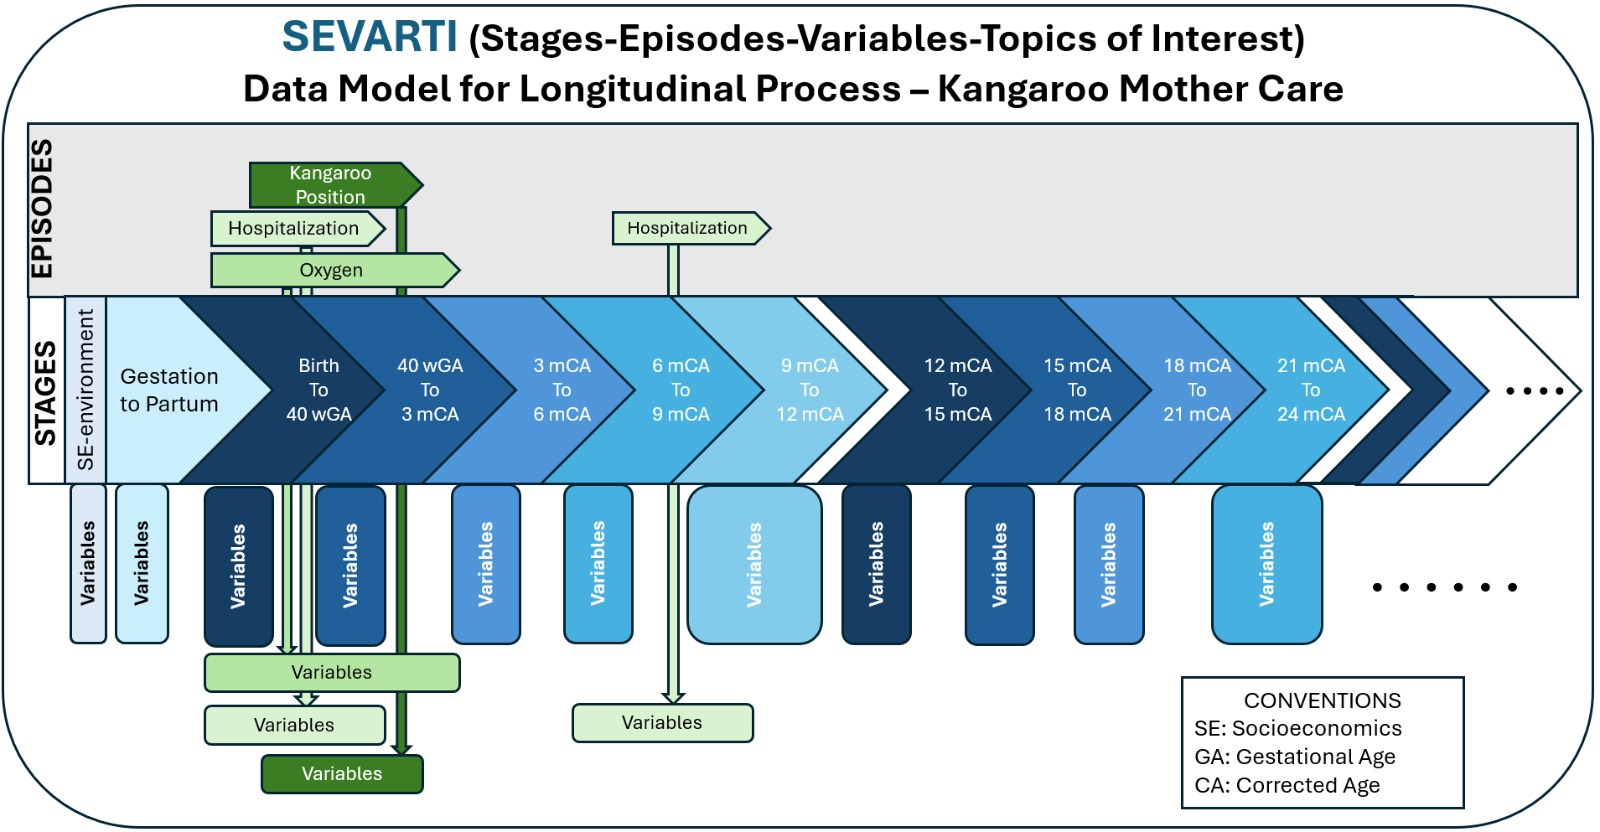
\includegraphics[width=\columnwidth]{figuras/sevarti.jpg}
\caption{Modelo conceptual SEVARTI del proceso longitudinal del Método Madre Canguro. \fuente{Fundación Canguro \cite{fundacion2026}.}}
\label{fig:sevarti}
\end{figure}

\textbf{Variables restringidas.} Durante el proyecto la Fundación restringió y luego liberó la sede y la fecha exacta de parto; la llave del paciente nunca se usa. El sistema trabaja sin sede ni fecha de parto (solo el año): la vigilancia temporal trata el programa como un solo grupo y la división de los datos es por año de nacimiento. El código queda listo para incorporarlas si la Fundación lo autoriza.

\textbf{División temporal.} Los niños se dividen por año de nacimiento, sin niño repetido entre partes y \emph{dentro de cada régimen} de registro (antes y después del cambio de sistema de 2022): los nacidos más recientes de cada régimen van a prueba. Dividir solo por fecha dejaría el régimen nuevo fuera del entrenamiento. Para el modelo de anomalías resultan 40.711 niños de entrenamiento, 7.330 de calibración y 8.955 de prueba; para el clínico, 48.041 de entrenamiento y los mismos 8.955 de prueba.

\subsection{Preprocesamiento: entrenar con datos sucios}
\label{sec:preproc}
Imputar esconde errores y limpiar de más convierte casos raros pero reales en alertas. Por eso ningún valor se imputa ni se corrige, y la base nunca se modifica. Cada dato se decide por separado: si se excluye, deja de ser objetivo y entra como faltante cuando es entrada de otra variable, lo que LightGBM maneja de forma nativa \cite{ke2017}. Se excluyen del entrenamiento los códigos especiales (que significan ``no se hizo''), los errores de unidad, los valores a más de 6 desviaciones robustas y, en una segunda vuelta, el peor 1\,\% de los residuos que superen 3,5. Los rangos del diccionario no se usan como filtro porque varios se calcularon de los mismos datos. Las exclusiones forman una máscara versionada; en el corte analizado suman el 1,6\,\% de los 3,53 millones de datos numéricos, y el 52\,\% de ellas son códigos especiales. El quiebre de 2022 entra como variable para que el modelo lo aprenda.

\subsection{Etapa 1: modelo de anomalías}
\label{sec:met-anomalias}
Una anomalía es un dato lejano de lo esperado para ese caso. El modelo tiene cinco capas, cada una con una pregunta distinta (Tabla~\ref{tab:capas}).

\begin{table}[t]
\centering
\caption{Capas del modelo de anomalías}
\label{tab:capas}
\footnotesize
\setlength{\tabcolsep}{3pt}
\begin{tabularx}{\columnwidth}{@{}l>{\raggedright\arraybackslash}X>{\raggedright\arraybackslash}X@{}}
\toprule
\textbf{Capa} & \textbf{Pregunta} & \textbf{Método} \\
\midrule
0. Contrato & ¿Cumple el esquema? & Tipo, variable conocida, fecha posible; si no, se rechaza \\
1. Valor & ¿Tiene sentido por sí solo? & $z$ robusto (mediana y MAD), códigos especiales, errores de unidad \\
2. Contexto & ¿Tiene sentido para este niño? & LightGBM por cuantiles por variable, con umbral conformal \\
3. Trayectoria & ¿Encaja con su historia? & Ventana de la etapa, orden, edad frente a fecha, talla que no baja, cambio frente a pares \\
4. Grupo y tiempo & ¿Algo empezó a medirse distinto? & Residuos, faltantes y redondeo por trimestre; CUSUM \\
\bottomrule
\end{tabularx}
\end{table}

La capa 1 usa $z = (x - \tilde{x})/(1{,}4826\,\mathrm{MAD})$ y alerta desde $|z| > 3{,}5$; un valor que aparece en más del 1\,\% de los datos no se considera raro. La capa 2 entrena, para cada variable numérica, tres modelos de regresión por cuantiles \cite{koenker1978} (0,25, 0,5 y 0,75) con la etapa, la edad cronológica y corregida, las covariables al nacer, el contexto socioeconómico, los episodios activos y las demás variables de la misma etapa. El residuo estandarizado es
\begin{equation}
z_2 = \frac{y - \hat{q}_{0{,}5}}{(\hat{q}_{0{,}75} - \hat{q}_{0{,}25})/1{,}349},
\label{eq:z2}
\end{equation}
y el umbral sale de la predicción conformal \cite{romano2019,angelopoulos2023}: en la partición de calibración se calcula el cuantil $1-\alpha$ de $|z_2|$, con $\alpha = 0{,}005$, de modo que en datos limpios salten unas 5 alertas por cada 1.000. Así el umbral se adapta a cada variable sin fijarlo a mano. Una variable nueva recibe modelo de capa 2 cuando reúne 200 niños, sin reentrenar las demás.

La capa 3 encadena por concepto (peso, talla, perímetro cefálico) las variables de distintas etapas y revisa la ventana de cada etapa, el orden de las visitas, la concordancia entre edad anotada y fecha (14 días de tolerancia), que la talla y el perímetro no bajen más de 1~cm, y el cambio entre visitas frente a los niños en la misma transición. La capa 4 compara cada trimestre con la mediana de los 8 anteriores en tres señales (residuo de la capa 2, proporción de faltantes y de valores redondeados) y acumula desvíos sostenidos con CUSUM \cite{page1954}:
\begin{equation}
S_t = \max\bigl(0,\, S_{t-1} + x_t - k\bigr), \quad \text{alarma si } S_t > h,
\label{eq:cusum}
\end{equation}
con $k = 0{,}5$ y $h = 8$, en ambas direcciones.

\subsection{Etapa 2: alertas clínicas}
\label{sec:met-clinico}
El modelo de anomalías no sirve para alertas clínicas: aprende lo normal de una base de niños prematuros, y un niño pequeño en todo le parece coherente. La segunda etapa usa los datos ya revisados (lo que la etapa 1 marca como código, error de unidad o valor a más de 6 MAD entra como faltante) y produce dos señales.

\textbf{Riesgo de un desenlace.} Se entrena un clasificador LightGBM por desenlace y momento de cálculo, con parada temprana. Los 14 desenlaces en uso son: readmisión en cinco ventanas (antes de las 40 semanas y entre visitas hasta los 12 meses), no volver a la siguiente visita (cinco momentos), oxigenodependencia con diagnóstico de displasia broncopulmonar o hipertensión pulmonar a los 3 y 12 meses, y desarrollo psicomotor bajo a los 6 y 12 meses, definido como el 10\,\% inferior del puntaje de los niños de entrenamiento porque el diccionario no identifica la escala. Cuatro desenlaces adicionales de crecimiento a los 12 meses (talla, peso, peso para la talla y perímetro cefálico por debajo de $-2$ DE) responden la pregunta original de la Fundación sobre malnutrición y se calculan desde las 40 semanas y los 3, 6 y 9 meses.

Tres decisiones evitan la fuga de información: (i) cada modelo solo ve datos de su visita o anteriores; (ii) se excluyen las variables que la base llena con retraso o solo cuando el niño vuelve, detectadas porque aparecen mucho menos en las visitas recientes y en los niños pendientes; y (iii) ``no volver'' solo cuenta si la ventana de la visita siguiente ya cerró. Las probabilidades se calibran con regresión isotónica sobre el 15\,\% de niños más recientes con desenlace conocido, que el modelo no vio, y se recalibran en cada entrenamiento \cite{vancalster2019}. Para cada niño se entrega el riesgo, su percentil frente a los niños de calibración y las tres variables que más lo suben según TreeSHAP \cite{lundberg2020}. El modelo no fija umbral: cuántos niños se muestran y desde qué riesgo lo decide la aplicación con el equipo clínico.

\textbf{Crecimiento frente a la OMS.} Desde las 40 semanas, peso, talla y perímetro cefálico se convierten en puntaje $z$ por edad corregida con el método LMS de los estándares de la OMS \cite{oms2006}:
\begin{equation}
z = \frac{(y/M)^{L} - 1}{L\,S},
\label{eq:lms}
\end{equation}
donde $L$, $M$ y $S$ dependen de la edad y el sexo. Se alerta por $z < -2$ y por una caída de más de 1 DE entre visitas; un valor biológicamente improbable se envía a revisión del dato y no al médico. En los resultados presentados se usó el límite simplificado $|z| > 6$; la versión final adopta los límites por indicador de la OMS \cite{omsunicef2019} \pendiente{actualizar cifras de la Tabla~\ref{tab:oms} con los límites exactos}. Antes de las 40 semanas no se evalúa crecimiento: el uso de una curva de prematuros \cite{fenton2013,villar2015} queda como trabajo futuro.

\subsection{Validación}
\label{sec:validacion}
\textbf{Anomalías.} Como no hay etiquetas de anomalía, se inyectan errores de seis tipos (unidad, código, dígitos invertidos, desvío de 3 DE, valor de otro niño y etapas intercambiadas) en datos limpios de la partición de prueba, cerca del 2\,\% de los datos por ronda en tres rondas, y se mide el porcentaje detectado frente a la regla vigente del rango del diccionario. Las falsas alertas se miden en la prueba sin errores inyectados. También se simula una báscula que suma un sesgo creciente desde una fecha y se mide cuántos trimestres tarda la alarma.

\textbf{Alertas clínicas.} En los niños de prueba se mide el AUC, el porcentaje de casos que queda en el 10\,\% de mayor riesgo y la razón entre riesgo medio y frecuencia observada, por desenlace y por subgrupos de edad gestacional e ingreso del hogar. La línea base es el mismo modelo con solo edad gestacional, peso al nacer y peso a la entrada. Como la revisión ciega por médicos no se pudo programar en el plazo del curso, el componente cualitativo se compone de dos análisis: un \emph{periodo en silencio retrospectivo}, que calcula los riesgos de los niños pendientes en un corte pasado y los compara con lo que ocurrió después, y un análisis de plausibilidad clínica de las variables que más pesan en cada desenlace. Se complementa con PR-AUC y días de anticipación, apropiados para desenlaces poco frecuentes.

\subsection{Herramientas y entorno de despliegue}
\label{sec:despliegue}
El sistema está escrito en Python, con pandas, NumPy, SciPy, LightGBM y PyArrow, y probado con pruebas automáticas sobre un simulador que genera tablas SEVARTI con los mismos problemas de la base real. La arquitectura (Fig.~\ref{fig:arquitectura}) sigue prácticas de MLOps \cite{kreuzberger2023}: una corrida semestral en contenedores Docker, programada para cuando la Fundación carga la base, ejecuta en orden el modelo de anomalías, su cola de revisión, el modelo clínico y el cálculo de riesgos (cerca de una hora en CPU); MLflow \cite{zaharia2018} registra experimentos, métricas y versiones con estados de evaluación y producción; una API FastAPI sirve inferencia a demanda sobre tablas SEVARTI, y un tablero React ofrece tres perfiles (administración de modelos, evaluación experta y visualización) con la línea temporal de cada niño seudonimizado y avisos por correo. Los mismos contenedores corren en dos entornos: una demostración pública en Railway con datos del simulador y una instalación interna con la base real en solo lectura, de modo que los datos por niño nunca salen del equipo.

% Figura: arquitectura de la solución (TikZ, legible en escala de grises)
\begin{figure*}[t]
\centering
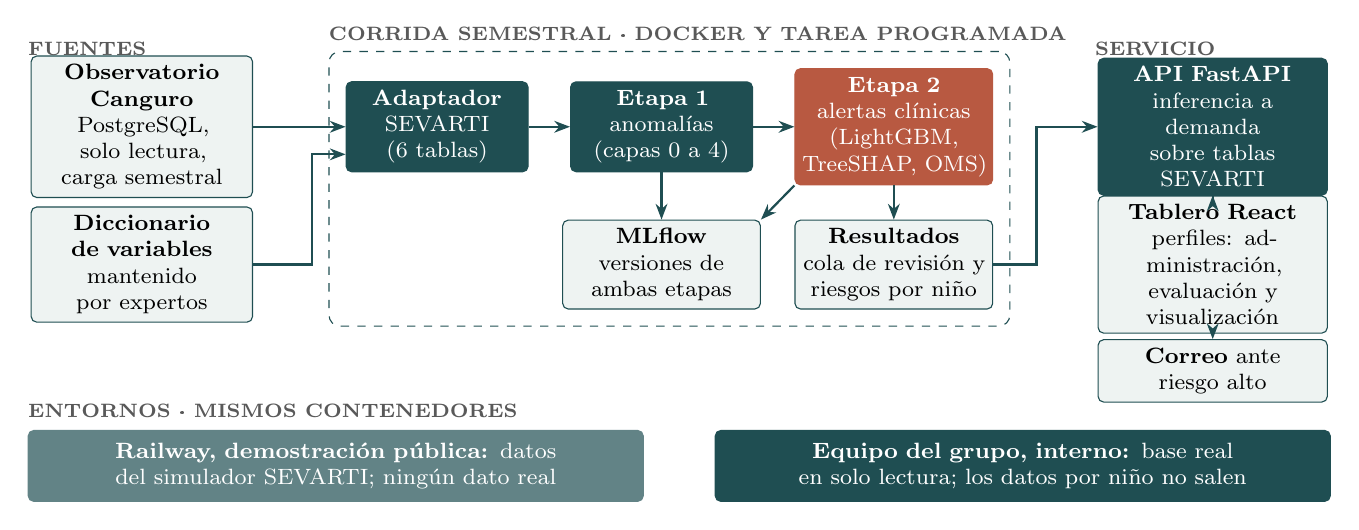
\begin{tikzpicture}[
  font=\footnotesize,
  >={Stealth[length=2mm]},
  caja/.style={draw=tinta, rounded corners=2pt, align=center, minimum height=11mm, inner sep=3pt, fill=niebla},
  oscura/.style={caja, fill=tinta, text=white},
  acento/.style={caja, fill=acento!85!black, draw=acento!85!black, text=white},
  rotulo/.style={font=\scriptsize\bfseries, text=black!65, inner sep=0pt},
  flecha/.style={->, draw=tinta, thick},
]
% --- Fuentes (columna izquierda)
\node[rotulo, anchor=south west] at (0,3.25) {FUENTES};
\node[caja, text width=26mm] (bd) at (1.45,2.35) {\textbf{Observatorio Canguro}\\PostgreSQL, solo lectura,\\carga semestral};
\node[caja, text width=26mm] (dic) at (1.45,0.6) {\textbf{Diccionario}\\\textbf{de variables}\\mantenido por expertos};

% --- Corrida semestral (centro)
\node[oscura, text width=21mm] (sev) at (5.2,2.35) {\textbf{Adaptador}\\SEVARTI\\(6 tablas)};
\node[oscura, text width=21mm] (ano) at (8.05,2.35) {\textbf{Etapa 1}\\anomalías\\(capas 0 a 4)};
\node[acento, text width=23mm] (cli) at (11.0,2.35) {\textbf{Etapa 2}\\alertas clínicas\\(LightGBM, TreeSHAP, OMS)};
\node[caja, text width=23mm] (mlf) at (8.05,0.6) {\textbf{MLflow}\\versiones de ambas etapas};
\node[caja, text width=23mm] (res) at (11.0,0.6) {\textbf{Resultados}\\cola de revisión y riesgos por niño};
\begin{scope}[on background layer]
\node[draw=tinta, dashed, rounded corners=4pt, fit=(sev)(ano)(cli)(mlf)(res), inner sep=6pt] (pipe) {};
\end{scope}
\node[rotulo, anchor=south west] at ([yshift=1.2mm]pipe.north west) {CORRIDA SEMESTRAL \textperiodcentered{} DOCKER Y TAREA PROGRAMADA};

% --- Servicio (columna derecha)
\node[rotulo, anchor=south west] at (13.55,3.25) {SERVICIO};
\node[oscura, text width=27mm] (api) at (15.05,2.35) {\textbf{API FastAPI}\\inferencia a demanda\\sobre tablas SEVARTI};
\node[caja, text width=27mm] (tab) at (15.05,0.6) {\textbf{Tablero React}\\perfiles: administración,\\evaluación y visualización};
\node[caja, text width=27mm, minimum height=7mm] (mail) at (15.05,-0.75) {\textbf{Correo} ante riesgo alto};

% --- Flechas
\draw[flecha] (bd) -- (sev);
\draw[flecha] (dic.east) -- ++(0.75,0) |- ([yshift=-3.5mm]sev.west);
\draw[flecha] (sev) -- (ano);
\draw[flecha] (ano) -- (cli);
\draw[flecha] (ano) -- (mlf);
\draw[flecha] (cli) -- (res);
\draw[flecha] (cli.south west) -- (mlf.north east);
\draw[flecha] (res.east) -- ++(0.55,0) |- (api.west);
\draw[flecha] (api) -- (tab);
\draw[flecha] (tab) -- (mail);

% --- Entornos
\node[rotulo, anchor=south west] at (0,-1.35) {ENTORNOS \textperiodcentered{} MISMOS CONTENEDORES};
\node[oscura, text width=76mm, minimum height=9mm, fill=tinta!70, draw=tinta!70, anchor=north west] (demo) at (0,-1.5) {\textbf{Railway, demostración pública:} datos del simulador SEVARTI; ningún dato real};
\node[oscura, text width=76mm, minimum height=9mm, anchor=north east] (int) at (16.55,-1.5) {\textbf{Equipo del grupo, interno:} base real en solo lectura; los datos por niño no salen};
\end{tikzpicture}
\caption{Arquitectura de la solución: fuentes, corrida semestral con las dos etapas (la etapa 2 recibe los datos ya revisados por la etapa 1), registro de modelos, servicio y entornos de despliegue. \fuente{elaboración propia.}}
\label{fig:arquitectura}
\end{figure*}


% ---------------------------------------------------------------------
% 4. Resultados  (criterio: Resultados, 15 pts)
%    Cifras del corte del 24/07/2026; modelo de anomalías 98aaa133d1.
% ---------------------------------------------------------------------
\section{Resultados}
\label{sec:resultados}

Todas las cifras corresponden al corte del 24 de julio de 2026 y se calculan en la partición de prueba, salvo que se indique otra cosa.

\subsection{Calidad y cobertura de la cohorte}
\label{sec:res-datos}
La base consultada tiene 4,0 veces más niños y 3,1 veces más mediciones que su documentación (15.641 niños y 4,5 millones de mediciones), por lo que toda cifra se reporta con su fecha de corte. El 76\,\% de las mediciones está marcado como ``sin ubicación temporal''; aun así, la edad anotada en cada visita coincide con la diferencia entre la fecha de la visita y la de parto en más del 99,7\,\% de los casos, lo que permitió construir el eje temporal. La Fig.~\ref{fig:cobertura} muestra la cobertura del peso entre los niños que ya tenían edad para cada visita: cae del 78\,\% a las 40 semanas al 49\,\% a los 12 meses. El peso al nacer solo se registra desde 2022, de ahí su baja cobertura.

% Figura: cobertura del peso entre los niños elegibles por visita
\begin{figure}[t]
\centering
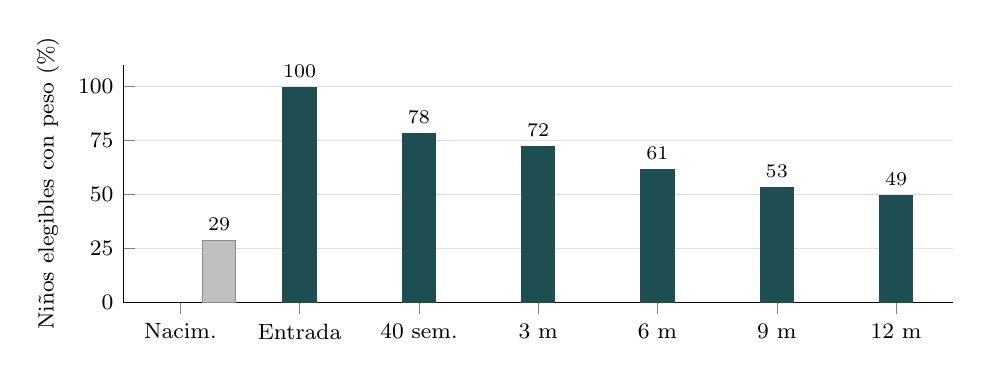
\begin{tikzpicture}
\begin{axis}[
  width=\columnwidth, height=4.6cm,
  ybar, bar width=12pt,
  ymin=0, ymax=110, ytick={0,25,50,75,100},
  ylabel={Niños elegibles con peso (\%)}, ylabel style={font=\footnotesize},
  symbolic x coords={Nacim.,Entrada,40 sem.,3 m,6 m,9 m,12 m},
  xtick={Nacim.,Entrada,40 sem.,3 m,6 m,9 m,12 m}, xticklabel style={font=\footnotesize},
  yticklabel style={font=\footnotesize},
  nodes near coords, nodes near coords style={font=\scriptsize, /pgf/number format/use comma, /pgf/number format/precision=0, /pgf/number format/fixed},
  axis lines*=left, ymajorgrids, grid style={black!12},
  enlarge x limits=0.08,
]
\addplot[fill=tinta, draw=tinta] coordinates {(Entrada,99.56) (40 sem.,78.01) (3 m,72.11) (6 m,61.33) (9 m,53.18) (12 m,49.37)};
\addplot[fill=black!25, draw=black!45, forget plot] coordinates {(Nacim.,28.65)};
\end{axis}
\end{tikzpicture}
\caption{Cobertura del peso entre los niños que ya tenían edad para cada visita. El nacimiento (gris) solo se registra desde 2022. \fuente{elaboración propia.}}
\label{fig:cobertura}
\end{figure}


Los hallazgos de calidad más relevantes fueron: 11 rangos del diccionario iguales al mínimo y máximo observados; 37 variables numéricas sin unidad; una unidad mal declarada (una variable en ``semanas'' que coincide con días en el 94,2\,\% de los casos); 8 variables que fallan su propia bandera de calidad en el 95\,\% o más de sus valores, por reglas mal configuradas; una talla al nacer que disminuye más de 1~cm al entrar al programa en el 34\,\% de los pares, señal de un instrumento distinto, y un aumento de pesos redondeados a 100~g del 0,9\,\% al 5,4\,\% tras el cambio de sistema de 2022.

\subsection{Modelo de anomalías}
\label{sec:res-anomalias}
El entrenamiento tomó 15,7 minutos en CPU y produjo 132 modelos de capa 2. La Fig.~\ref{fig:errores} compara el porcentaje de errores inyectados que detecta el modelo (cualquier capa) con el de la regla del rango del diccionario. El modelo detecta entre el 34\,\% y el 99\,\% según el tipo, frente a entre el 1\,\% y el 97\,\% de la regla vigente. La mayor ganancia está en los errores plausibles en sí mismos: un desvío de 3 DE pasa del 27\,\% al 78\,\%, y las etapas intercambiadas, del 5\,\% al 68\,\%. En los desvíos de 3 DE, la capa 1 detecta el 31\,\% y la capa 2 el 68\,\%; esa diferencia mide el aporte del contexto. El tipo más difícil es el valor de otro niño (34\,\%), porque solo se nota cuando choca con el resto de la información.

% Figura: errores inyectados detectados por tipo, modelo frente a la regla vigente
\begin{figure}[t]
\centering
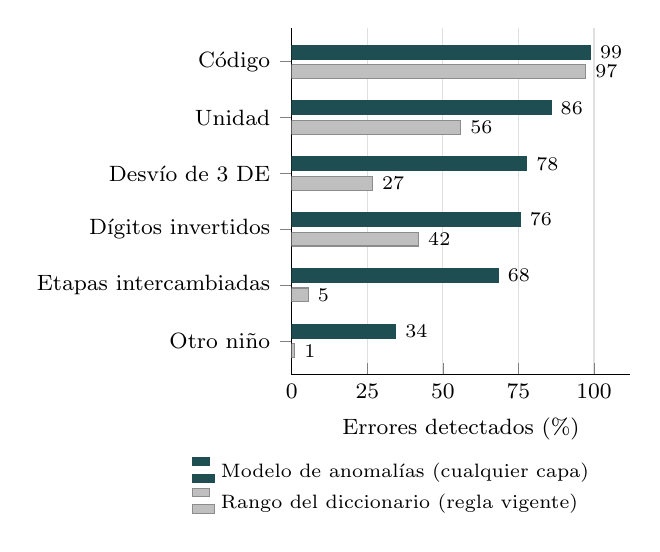
\begin{tikzpicture}
\begin{axis}[
  scale only axis, width=4.3cm, height=4.4cm,
  xbar, bar width=5pt,
  xmin=0, xmax=112, xtick={0,25,50,75,100},
  xlabel={Errores detectados (\%)}, xlabel style={font=\footnotesize},
  symbolic y coords={Otro niño,Etapas intercambiadas,Dígitos invertidos,Desvío de 3 DE,Unidad,Código},
  ytick=data, yticklabel style={font=\footnotesize},
  xticklabel style={font=\footnotesize},
  nodes near coords, nodes near coords style={font=\scriptsize, /pgf/number format/use comma, /pgf/number format/precision=0, /pgf/number format/fixed},
  axis lines*=left, xmajorgrids, grid style={black!12},
  enlarge y limits=0.12,
  legend style={font=\scriptsize, at={(0.3,-0.22)}, anchor=north, draw=none, legend columns=1},
  legend cell align=left,
  reverse legend,
]
\addplot[fill=black!25, draw=black!45] coordinates {(0.92,Otro niño) (5.44,Etapas intercambiadas) (41.93,Dígitos invertidos) (26.65,Desvío de 3 DE) (55.83,Unidad) (97.24,Código)};
\addplot[fill=tinta, draw=tinta] coordinates {(34.33,Otro niño) (68.30,Etapas intercambiadas) (75.55,Dígitos invertidos) (77.69,Desvío de 3 DE) (85.76,Unidad) (98.77,Código)};
\legend{Rango del diccionario (regla vigente), Modelo de anomalías (cualquier capa)}
\end{axis}
\end{tikzpicture}
\caption{Porcentaje de errores inyectados que se detectan, por tipo de error, en la partición de prueba. \fuente{elaboración propia.}}
\label{fig:errores}
\end{figure}


En datos limpios, el modelo emite 18,8 alertas por cada 1.000 datos (capa 1: 4,4; capa 2: 8,9; capa 3: 7,2), frente a 14,7 de la regla vigente. La curva de $\alpha$ muestra el compromiso: con $\alpha = 0{,}001$ se emitirían 15,2 alertas por 1.000 y se detectaría el 72,7\,\% de los errores; con el valor adoptado, $\alpha = 0{,}005$, 18,8 y 75,3\,\%. La capa 2 alerta por encima de su meta (8,9 frente a 5) porque parte de los datos ``limpios'' son errores reales no marcados; solo la revisión experta puede separarlos.

En la vigilancia temporal, un sesgo de báscula del tamaño de una escala de la capa 2 (unos 407~g en el peso de los 3 meses) dispara la alarma en el mismo trimestre en que empieza, con 3 alarmas falsas en el periodo sin sesgo. Al agregar una variable nueva (simulada con una talla), las capas 1 y 3 la revisan desde el primer dato y su modelo de capa 2 se entrena en 45 segundos sin cambiar los otros 131. Sobre toda la historia, el modelo envía a revisión 105.313 datos (19,4 por 1.000) de 38.466 niños; la tasa anual cae de 41,3 por 1.000 antes de 2022 a 13,0 después, coherente con un sistema de registro más controlado.

\subsection{Alertas clínicas}
\label{sec:res-clinico}
Entrenar los 14 modelos tomó 3,5 minutos. Se excluyeron tres variables de llenado tardío; antes de quitarlas, el 62\,\% de los niños pendientes de la visita de 6 meses quedaba en el 10\,\% de mayor riesgo de no volver, un artefacto de fuga de información. De los 56.910 niños que entran al programa con fecha, el 7,5\,\% de los que ya debían volver a las 40 semanas no volvió.

La Tabla~\ref{tab:clinico} resume la validación. El modelo supera a la regla simple en AUC en 13 de los 14 desenlaces y empata en el restante (oxigenodependencia a los 12 meses, 0,76). El mejor desempeño es la oxigenodependencia con diagnóstico a los 3 meses (AUC 0,91; 68\,\% de los casos en el 10\,\% de mayor riesgo, frente a 49\,\% de la regla) y el desarrollo psicomotor bajo (AUC 0,71 y 0,77; 35--39\,\% de los casos arriba frente a 20--24\,\%). ``No volver'' desde los 3 meses y la readmisión tardía apenas se anticipan (AUC 0,56--0,65).

\begin{table*}[t]
\centering
\caption{Validación de las alertas clínicas en los niños de prueba (no vistos por el modelo)}
\label{tab:clinico}
\footnotesize
\setlength{\tabcolsep}{4pt}
\resizebox{\textwidth}{!}{%
\begin{tabular}{@{}llrrcccccc@{}}
\toprule
& & & & \multicolumn{2}{c}{\textbf{AUC}} & \multicolumn{2}{c}{\textbf{Casos en el 10\,\% superior (\%)}} & \textbf{Riesgo medio /} \\
\cmidrule(lr){5-6}\cmidrule(lr){7-8}
\textbf{Desenlace} & \textbf{Se calcula en} & \textbf{Niños} & \textbf{Casos (\%)} & \textbf{Modelo} & \textbf{Regla} & \textbf{Modelo} & \textbf{Regla} & \textbf{observado} \\
\midrule
Readmisión antes de 40 semanas & Entrada & 6.323 & 4,90 & 0,71 & 0,67 & 29,7 & 28,1 & 1,64 \\
Readmisión 40 semanas--3 meses & 40 semanas & 3.886 & 3,68 & 0,67 & 0,58 & 22,4 & 23,1 & 1,39 \\
Readmisión 3--6 meses & 3 meses & 3.385 & 1,60 & 0,62 & 0,53 & 16,7 & 18,5 & 2,96 \\
Readmisión 6--9 meses & 6 meses & 2.615 & 1,99 & 0,57 & 0,48 & 15,4 & 11,5 & 1,59 \\
Readmisión 9--12 meses & 9 meses & 2.295 & 1,57 & 0,65 & 0,50 & 19,4 & 13,9 & 2,01 \\
\midrule
No vuelve a 40 semanas & Entrada & 2.222 & 10,80 & 0,67 & 0,57 & 25,0 & 13,8 & 0,98 \\
No vuelve a 3 meses & 40 semanas & 4.338 & 17,73 & 0,67 & 0,53 & 19,9 & 12,7 & 0,97 \\
No vuelve a 6 meses & 3 meses & 4.660 & 29,55 & 0,56 & 0,49 & 13,1 & 9,6 & 0,90 \\
No vuelve a 9 meses & 6 meses & 3.855 & 34,03 & 0,57 & 0,52 & 13,4 & 10,0 & 0,84 \\
No vuelve a 12 meses & 9 meses & 3.150 & 29,71 & 0,58 & 0,52 & 14,7 & 10,7 & 1,06 \\
\midrule
Oxigenodependencia a 3 meses & Entrada & 5.315 & 3,78 & \textbf{0,91} & 0,80 & \textbf{67,7} & 49,3 & 1,58 \\
Oxigenodependencia a 12 meses & 40 semanas & 2.140 & 0,98 & 0,76 & 0,76 & 57,1 & 33,3 & 0,98 \\
Desarrollo psicomotor bajo a 6 meses & 3 meses & 3.187 & 4,42 & 0,71 & 0,57 & 35,5 & 19,9 & 0,99 \\
Desarrollo psicomotor bajo a 12 meses & 6 meses & 2.343 & 4,65 & 0,77 & 0,59 & 39,5 & 23,9 & 0,91 \\
\bottomrule
\end{tabular}}
\par\vspace{2pt}\raggedright\scriptsize Regla: el mismo modelo con solo edad gestacional, peso al nacer y peso a la entrada. Una razón riesgo/observado mayor que 1 indica sobreestimación. \fuente{elaboración propia.}
\end{table*}

Discriminar no es lo mismo que acertar el nivel. En 8 de los 14 desenlaces el riesgo medio está entre 0,8 y 1,25 veces lo observado, pero en 6 lo sobreestima, sobre todo en la readmisión de 3 a 6 meses (2,96 veces): los nacidos más recientes tienen menos eventos que los niños con que se calibró. El mismo patrón aparece por subgrupos: en la readmisión antes de las 40 semanas, el riesgo medio es 13,2\,\% frente a 8,0\,\% observado en menores de 32 semanas, 8,7\,\% frente a 5,4\,\% entre 32 y 36, y 6,2\,\% frente a 3,6\,\% en 37 o más; el orden entre grupos se conserva y el nivel se desplaza de forma pareja. Por ingreso del hogar la sobreestimación es mayor en el grupo de ingreso bajo (7,7\,\% frente a 3,3\,\%).

En PR-AUC y días de anticipación: \pendiente{agregar PR-AUC por desenlace y la mediana de días entre el cálculo del riesgo y el evento}.

\subsection{Crecimiento frente a la OMS}
\label{sec:res-oms}
La Tabla~\ref{tab:oms} resume el crecimiento desde las 40 semanas. La talla es el indicador más afectado (mediana de $z$ entre $-1{,}20$ y $-1{,}05$; 19--22\,\% por debajo de $-2$ DE), seguida del peso (11--12\,\%), mientras el perímetro cefálico se mantiene cerca de la mediana de la OMS. En total, 60.315 datos quedan por debajo de $-2$ DE o caen más de 1 DE entre visitas, y 770 superan el límite de dato improbable y se envían a revisión. La caída de más de 1 DE, máxima a los 3 meses (5,9\,\% de los pesos), aparece antes de que el niño cruce $-2$ DE, y es una señal que el modelo de anomalías nunca habría dado, porque en esta cohorte es común.

\begin{table}[t]
\centering
\caption{Crecimiento frente a los estándares de la OMS por visita}
\label{tab:oms}
\footnotesize
\setlength{\tabcolsep}{3pt}
\begin{tabular}{@{}llrrrr@{}}
\toprule
\textbf{Visita} & \textbf{Indicador} & \textbf{Datos} & \textbf{$z$ med.} & \textbf{$<-2$ DE} & \textbf{Cae $>1$ DE} \\
\midrule
\multirow{3}{*}{40 sem.} & Peso & 24.120 & $-0{,}91$ & 11,7 & 0,3 \\
 & Talla & 20.243 & $-1{,}11$ & 20,5 & 0,0 \\
 & P. cefálico & 6.323 & 0,53 & 1,1 & 0,0 \\
\midrule
\multirow{3}{*}{3 meses} & Peso & 39.881 & $-0{,}66$ & 10,6 & 5,9 \\
 & Talla & 39.808 & $-1{,}20$ & 22,4 & 5,5 \\
 & P. cefálico & 39.712 & 0,05 & 4,2 & 2,3 \\
\midrule
\multirow{3}{*}{6 meses} & Peso & 33.067 & $-0{,}73$ & 12,0 & 3,6 \\
 & Talla & 33.065 & $-1{,}14$ & 20,4 & 5,0 \\
 & P. cefálico & 33.011 & 0,08 & 3,3 & 3,6 \\
\midrule
\multirow{3}{*}{9 meses} & Peso & 28.231 & $-0{,}67$ & 11,5 & 1,8 \\
 & Talla & 28.153 & $-1{,}05$ & 18,9 & 3,8 \\
 & P. cefálico & 28.176 & 0,14 & 3,3 & 3,0 \\
\midrule
\multirow{3}{*}{12 meses} & Peso & 25.660 & $-0{,}65$ & 10,7 & 1,4 \\
 & Talla & 25.633 & $-1{,}06$ & 18,6 & 3,3 \\
 & P. cefálico & 25.625 & 0,20 & 3,7 & 2,6 \\
\bottomrule
\end{tabular}
\par\vspace{2pt}\raggedright\scriptsize Porcentajes de los datos de cada fila; $z$ por edad corregida (LMS). \fuente{elaboración propia.}
\end{table}

\textbf{Desenlaces de crecimiento a los 12 meses.} \pendiente{tabla con AUC, AUC de la regla y casos en el 10\,\% de mayor riesgo para talla baja, peso bajo, desnutrición aguda (peso para la talla) y perímetro cefálico bajo a los 12 meses, calculados desde las 40 semanas y los 3, 6 y 9 meses}.

\subsection{Validación retrospectiva y plausibilidad de las explicaciones}
\label{sec:res-silencio}
\pendiente{periodo en silencio retrospectivo: corte usado, niños pendientes en ese corte, AUC, calibración y casos en el 10\,\% de mayor riesgo frente a lo ocurrido después, por desenlace}.

\pendiente{análisis de plausibilidad: las variables con mayor contribución TreeSHAP por desenlace, contrastadas con la literatura clínica, y dos o tres casos anonimizados con su ``porqué''}.

\subsection{Despliegue}
\label{sec:res-despliegue}
\pendiente{resultados del despliegue: corridas completas exitosas y su duración, tiempo de respuesta de la API por niño y por lote, pruebas automáticas aprobadas, pruebas de los tres perfiles y del correo, y captura del tablero con la línea temporal de un niño simulado}.

% ---------------------------------------------------------------------
% 5. Discusión y aportes  (criterio: Discusión y aportes, 15 pts)
%    Interpretación crítica, aportes, limitaciones y posibles aplicaciones.
% ---------------------------------------------------------------------
\section{Discusión y aportes}
\label{sec:discusion}

\textbf{Interpretación.} Los resultados respaldan la separación en dos etapas. El modelo de anomalías gana sobre todo en los errores que son plausibles por sí solos (desvíos, etapas intercambiadas), que ninguna regla de rangos puede ver; ese es el aporte del contexto del niño, y coincide con la crítica de que los marcos de calidad basados en reglas fijas ignoran al paciente \cite{kahn2016,weiskopf2013}. El costo es moderado: 4,1 alertas más por cada 1.000 datos limpios que la regla vigente, una parte de las cuales son errores reales todavía sin etiqueta.

En la etapa clínica, el desempeño sigue la naturaleza de cada desenlace. Los que dependen del estado biológico registrado al nacer y en la hospitalización (oxigenodependencia, desarrollo psicomotor) se anticipan bien y con ventaja clara sobre la regla. Los que dependen de factores que la base apenas registra (no volver a una cita desde los 3 meses, readmisiones tardías) se anticipan poco: el AUC cercano a 0,6 indica que esa información no está en los datos, no solo que el modelo sea débil. La discrepancia en dos readmisiones tempranas, con mejor AUC pero menos casos en el decil superior que la regla, recuerda que el AUC resume todo el orden mientras que el uso clínico mira solo la parte alta; por eso el sistema no fija un umbral y reporta ambas medidas. La sobreestimación en 6 de 14 desenlaces es deriva temporal \cite{davis2017}: el orden se conserva y el nivel se desplaza. Confirma la decisión de recalibrar en cada entrenamiento y de no mostrar porcentajes a los médicos antes del periodo en silencio \cite{vancalster2019,wong2021}.

\textbf{Aportes.} (i) Un sistema genérico guiado por un diccionario que gobiernan los expertos: agregar o retirar una variable no requiere cambiar código, y la entrada SEVARTI admite otras fuentes. (ii) La integración del dato con el niño: el modelo clínico aprende de datos revisados, y las alertas de crecimiento con un patrón externo (la OMS) cubren lo que un modelo entrenado en prematuros consideraría normal. (iii) Hallazgos de gobierno del dato ya entregados a la Fundación: rangos y unidades erróneos y la exposición de una llave de paciente, que se retiró. (iv) Una ruta de despliegue que mantiene los datos por niño dentro del equipo.

\textbf{Posibles aplicaciones.} La Tabla~\ref{tab:usos} resume cómo puede usar la Fundación cada resultado. Todas son apoyo a la decisión: el modelo ordena a los niños y explica por qué; la decisión de a quién llamar o remitir sigue en manos del equipo clínico.

\begin{table}[t]
\centering
\caption{Resultados y su uso potencial en el programa}
\label{tab:usos}
\footnotesize
\setlength{\tabcolsep}{3pt}
\begin{tabularx}{\columnwidth}{@{}>{\raggedright\arraybackslash}p{2.3cm}>{\raggedright\arraybackslash}X>{\raggedright\arraybackslash}p{1.7cm}@{}}
\toprule
\textbf{Resultado} & \textbf{Uso potencial} & \textbf{Quién} \\
\midrule
Cola de revisión de datos & Depurar cada carga semestral antes de analizar o publicar & Analítica \\
Defectos del diccionario & Corregir rangos, unidades y validaciones del formulario & Observatorio \\
Alarmas por trimestre & Auditar equipos y procesos; evaluar cambios de sistema & Coordinación \\
Riesgo de no volver & Priorizar recordatorios antes de la cita (ordena, no decide) & Seguimiento \\
Oxigenodependencia & Planear seguimiento respiratorio desde la entrada & Pediatría \\
Desarrollo bajo & Remitir antes a valoración del neurodesarrollo & Neurodesarrollo \\
Caída de $z$ OMS & Alerta nutricional antes de cruzar $-2$ DE & Pediatría, nutrición \\
\bottomrule
\end{tabularx}
\end{table}

\textbf{Limitaciones.} Primero, la \emph{pérdida de seguimiento}: solo el 46\,\% llega a los 12 meses, de modo que los desenlaces tardíos se conocen solo en quienes vuelven y pueden estar sesgados; por eso no volver se modela como desenlace propio. Segundo, la \emph{deriva}, ya discutida. Tercero, sin sede ni fecha de parto, la vigilancia temporal ve el programa como un todo y un cambio en una sola sede se diluye; tampoco es posible evaluar el desempeño por sede. Cuarto, el desarrollo ``bajo'' es relativo (10\,\% inferior), no un corte clínico. Quinto, antes de las 40 semanas no se evalúa crecimiento. Sexto, los errores inyectados miden solo los errores que se nos ocurren, y la validación clínica es retrospectiva: falta una evaluación prospectiva con neonatólogos.

\textbf{Consideraciones éticas.} El sistema es de apoyo y no emite diagnósticos \cite{salih2024}. Los datos están seudonimizados, no se intenta reidentificar, el repositorio no contiene datos por niño y la demostración pública usa datos simulados. Los sesgos se vigilan por edad gestacional e ingreso, y se reportan las limitaciones conforme a TRIPOD+AI \cite{collins2024}. Las explicaciones TreeSHAP describen asociaciones aprendidas, no causas \cite{ghassemi2021}, y así se presentan en el tablero.

% ---------------------------------------------------------------------
% 6. Conclusiones y trabajo futuro  (criterio: 10 pts)
% ---------------------------------------------------------------------
\section{Conclusiones y trabajo futuro}
\label{sec:conclusiones}

Este trabajo construyó y validó, sobre 62.043 niños del Observatorio Canguro, un sistema de inteligencia artificial interpretable de dos etapas. Respecto a la pregunta planteada, se concluye que: (i) la calidad del dato es un problema de primer orden y un modelo con contexto detecta el 75\,\% de los errores inyectados, con ganancias grandes donde las reglas de rango fallan; (ii) los riesgos calibrados superan a una regla simple en 13 de 14 desenlaces y son útiles cuando el desenlace depende del estado clínico registrado (oxigenodependencia, desarrollo psicomotor), pero no cuando depende de factores que la base no recoge (no volver al seguimiento); (iii) la comparación con la OMS revela que una de cada cinco tallas está por debajo de $-2$ DE durante el primer año y que la caída de más de 1 DE es una señal más temprana; y (iv) la calibración se desplaza con el tiempo, por lo que la recalibración y la evaluación en silencio son parte del sistema y no un paso opcional. \pendiente{completar con los hallazgos del periodo en silencio retrospectivo, los desenlaces de crecimiento a 12 meses y el despliegue}.

Como trabajo futuro se proponen: un periodo en silencio prospectivo con la siguiente carga semestral de la base y la revisión ciega por neonatólogos; la incorporación de la sede y la fecha de parto, si la Fundación lo autoriza, para vigilar cada sede contra su propio pasado; curvas de prematuros (Fenton o INTERGROWTH-21st) para evaluar el crecimiento antes de las 40 semanas; el análisis de trayectorias y firmas longitudinales de crecimiento, pregunta original de la Fundación, sobre los datos ya depurados; la integración del servicio con la aplicación del Observatorio; y la validación en otros Programas Madre Canguro.


\section*{Agradecimientos}
Agradecemos a la Fundación Canguro, y en particular al Prof. José Tiberio Hernández, responsable de Analítica, por el acceso al Observatorio Canguro y el acompañamiento durante el proyecto.

% Generado por herramientas/ordenar_referencias.py: no editar a mano.
% Orden de primera cita (IEEE).
\begin{thebibliography}{35}
\bibitem{oms2022}
World Health Organization, \emph{WHO Recommendations for Care of the Preterm or Low-Birth-Weight Infant}. Geneva: WHO, 2022.

\bibitem{victora2021}
C.~G. Victora, P. Christian, L.~P. Vidaletti, G. Gatica-Domínguez, P. Menon, and R.~E. Black, ``Revisiting maternal and child undernutrition in low-income and middle-income countries: variable progress towards an unfinished agenda,'' \emph{The Lancet}, vol.~397, no.~10282, pp.~1382--1396, 2021.

\bibitem{fundacion2026}
Fundación Canguro, ``Proyecto final de la maestría en Inteligencia Artificial: Crecimiento y riesgos en el niño prematuro o de bajo peso al nacer (KMC-12mCA-Growing and Risks),'' propuesta y documentación institucional, 2026.

\bibitem{charpak2017}
N. Charpak, R. Tessier, J.~G. Ruiz \emph{et al.}, ``Twenty-year follow-up of kangaroo mother care versus traditional care,'' \emph{Pediatrics}, vol.~139, no.~1, e20162063, 2017.

\bibitem{charpak2023}
N. Charpak and A. Montealegre-Pomar, ``Follow-up of Kangaroo Mother Care programmes in the last 28 years: results from a cohort of 57\,154 low-birth-weight infants in Colombia,'' \emph{BMJ Global Health}, vol.~8, no.~5, 2023.

\bibitem{fenton2013}
T.~R. Fenton and J.~H. Kim, ``A systematic review and meta-analysis to revise the Fenton growth chart for preterm infants,'' \emph{BMC Pediatrics}, vol.~13, art.~59, 2013.

\bibitem{villar2015}
J. Villar, F. Giuliani, Z.~A. Bhutta \emph{et al.}, ``Postnatal growth standards for preterm infants: the Preterm Postnatal Follow-up Study of the INTERGROWTH-21st Project,'' \emph{The Lancet Global Health}, vol.~3, no.~11, pp.~e681--e691, 2015, doi: 10.1016/S2214-109X(15)00163-1.

\bibitem{oms2006}
World Health Organization, \emph{WHO Child Growth Standards: Length/Height-for-Age, Weight-for-Age, Weight-for-Length, Weight-for-Height and Body Mass Index-for-Age: Methods and Development}. Geneva: WHO, 2006.

\bibitem{ren2024}
Z. Ren, W. Gao, Q. Wang \emph{et al.}, ``Predictive role of NICU-related stress, postpartum depression trajectory and family coping on growth trajectory of moderate-to-late preterm infants: A longitudinal study,'' \emph{Journal of Advanced Nursing}, vol.~80, no.~8, pp.~3167--3178, 2024, doi: 10.1111/jan.16068.

\bibitem{nel2026}
S. Nel, U.~D. Feucht, T. Botha, M. Arashi, and F.~A.~M. Wenhold, ``First-year growth patterns of preterm infants receiving kangaroo mother care: associations with early life factors and 1-year anthropometry,'' \emph{European Journal of Clinical Nutrition}, vol.~80, pp.~62--72, 2026, doi: 10.1038/s41430-025-01662-6.

\bibitem{melo2016}
S.~E. Melo, O.~O. Melo, and N. Suarez, ``Modelo multinivel de tasa global de ganancia de peso en el programa madre canguro en Bogotá,'' \emph{Revista de Salud Pública}, vol.~18, no.~2, pp.~238--250, 2016, doi: 10.15446/rsap.v18n2.44661.

\bibitem{baker2023}
S. Baker and Y. Kandasamy, ``Machine learning for understanding and predicting neurodevelopmental outcomes in premature infants: a systematic review,'' \emph{Pediatric Research}, vol.~93, pp.~293--299, 2023.

\bibitem{demirci2024}
G.~M. Demirci \emph{et al.}, ``Predicting mental and psychomotor delay in very pre-term infants using machine learning,'' \emph{Pediatric Research}, vol.~95, pp.~668--678, 2024.

\bibitem{mlrisk2024}
``Machine learning risk stratification for high-risk infant follow-up of term and late preterm infants,'' \emph{Pediatric Research}, 2024, doi: 10.1038/s41390-024-03338-6.

\bibitem{wang2024}
L.-Y. Wang, L.-Y. Wang, M.-I. Sung \emph{et al.}, ``Implementing explainable machine learning models for practical prediction of early neonatal hypoglycemia,'' \emph{Diagnostics}, vol.~14, no.~14, art.~1571, 2024, doi: 10.3390/diagnostics14141571.

\bibitem{kahn2016}
M.~G. Kahn, T.~J. Callahan, J. Barnard \emph{et al.}, ``A harmonized data quality assessment terminology and framework for the secondary use of electronic health record data,'' \emph{eGEMs}, vol.~4, no.~1, art.~1244, 2016, doi: 10.13063/2327-9214.1244.

\bibitem{weiskopf2013}
N.~G. Weiskopf and C. Weng, ``Methods and dimensions of electronic health record data quality assessment: enabling reuse for clinical research,'' \emph{Journal of the American Medical Informatics Association}, vol.~20, no.~1, pp.~144--151, 2013.

\bibitem{chandola2009}
V. Chandola, A. Banerjee, and V. Kumar, ``Anomaly detection: A survey,'' \emph{ACM Computing Surveys}, vol.~41, no.~3, art.~15, 2009.

\bibitem{koenker1978}
R. Koenker and G. Bassett, ``Regression quantiles,'' \emph{Econometrica}, vol.~46, no.~1, pp.~33--50, 1978.

\bibitem{romano2019}
Y. Romano, E. Patterson, and E. Candès, ``Conformalized quantile regression,'' in \emph{Advances in Neural Information Processing Systems}, vol.~32, 2019.

\bibitem{angelopoulos2023}
A.~N. Angelopoulos and S. Bates, ``Conformal prediction: A gentle introduction,'' \emph{Foundations and Trends in Machine Learning}, vol.~16, no.~4, pp.~494--591, 2023.

\bibitem{vancalster2019}
B. Van Calster, D.~J. McLernon, M. van Smeden, L. Wynants, and E.~W. Steyerberg, ``Calibration: the Achilles heel of predictive analytics,'' \emph{BMC Medicine}, vol.~17, art.~230, 2019.

\bibitem{davis2017}
S.~E. Davis, T.~A. Lasko, G. Chen, and M.~E. Matheny, ``Calibration drift among regression and machine learning models for hospital mortality,'' in \emph{AMIA Annual Symposium Proceedings}, vol.~2017, pp.~625--634, 2017.

\bibitem{wong2021}
A. Wong, E. Otles, J.~P. Donnelly \emph{et al.}, ``External validation of a widely implemented proprietary sepsis prediction model in hospitalized patients,'' \emph{JAMA Internal Medicine}, vol.~181, no.~8, pp.~1065--1070, 2021, doi: 10.1001/jamainternmed.2021.2626.

\bibitem{page1954}
E.~S. Page, ``Continuous inspection schemes,'' \emph{Biometrika}, vol.~41, no.~1/2, pp.~100--115, 1954.

\bibitem{lundberg2020}
S.~M. Lundberg, G. Erion, H. Chen \emph{et al.}, ``From local explanations to global understanding with explainable AI for trees,'' \emph{Nature Machine Intelligence}, vol.~2, no.~1, pp.~56--67, 2020.

\bibitem{salih2024}
A.~M. Salih, G. Menegaz, T. Pillay, and E.~M. Boyle, ``Explainable artificial intelligence in paediatric: Challenges for the future,'' \emph{Health Science Reports}, vol.~7, no.~12, e70271, 2024, doi: 10.1002/hsr2.70271.

\bibitem{ghassemi2021}
M. Ghassemi, L. Oakden-Rayner, and A.~L. Beam, ``The false hope of current approaches to explainable artificial intelligence in health care,'' \emph{The Lancet Digital Health}, vol.~3, no.~11, pp.~e745--e750, 2021.

\bibitem{collins2024}
G.~S. Collins, K.~G.~M. Moons, P. Dhiman \emph{et al.}, ``TRIPOD+AI statement: updated guidance for reporting clinical prediction models that use regression or machine learning methods,'' \emph{BMJ}, vol.~385, e078378, 2024.

\bibitem{kreuzberger2023}
D. Kreuzberger, N. Kühl, and S. Hirschl, ``Machine learning operations (MLOps): Overview, definition, and architecture,'' \emph{IEEE Access}, vol.~11, pp.~31866--31879, 2023, doi: 10.1109/ACCESS.2023.3262138.

\bibitem{zaharia2018}
M. Zaharia, A. Chen, A. Davidson \emph{et al.}, ``Accelerating the machine learning lifecycle with MLflow,'' \emph{IEEE Data Engineering Bulletin}, vol.~41, no.~4, pp.~39--45, 2018.

\bibitem{designcouncil2007}
Design Council, \emph{Eleven Lessons: Managing Design in Eleven Global Companies}. London: Design Council, 2007.

\bibitem{brown2008}
T. Brown, ``Design thinking,'' \emph{Harvard Business Review}, vol.~86, no.~6, pp.~84--92, 2008.

\bibitem{ke2017}
G. Ke, Q. Meng, T. Finley \emph{et al.}, ``LightGBM: A highly efficient gradient boosting decision tree,'' in \emph{Advances in Neural Information Processing Systems}, vol.~30, pp.~3146--3154, 2017.

\bibitem{omsunicef2019}
World Health Organization and UNICEF, \emph{Recommendations for Data Collection, Analysis and Reporting on Anthropometric Indicators in Children under 5 Years Old}. Geneva: WHO, 2019.

\end{thebibliography}


\end{document}
